\documentclass[asi]{picINSA}
\usepackage{lmodern}
\usepackage{amsmath}
\usepackage{amssymb}
\usepackage{mathrsfs}

% Bout de code pour enlever le ``chapitre'' écrit à chaque fois
\makeatletter
\def\@makechapterhead#1{
  {\parindent \z@ \raggedright \normalfont
    \interlinepenalty\@M
    \Huge\bfseries  \thechapter.\quad #1\par\nobreak
    \vskip 40\p@
  }}
\makeatother
% Enlève les doubles pages blanches inutiles
\let\cleardoublepage\clearpage


\begin{document}

    \titreGeneral{Sujet RPG1 \newline Manuel d'installation et d'utilisation}
	\sousTitreGeneral{\newline Sylvain GUINGOIN, Maxime PATTYN, \newline Claire RIVOIRE, Pierre SASSOULAS}
	\titreAcronyme{\LARGE IHME}
	\version{1.00}
	\referenceVersion{bibliographie}
	
	\couverture{}

\tableofcontents{}


\chapter{Installation}

L'installation du programme nécessite d'avoir le jre7 installé. \\

Pour compiler les fichiers sources, il suffit de se placer dans répertoire contenant le fichier \verb+build.xml+ et de lancer la commande : \verb+ant+. \\ 

Pour lancer le programme, il faut se placer dans le répertoire \verb+bin+ et lancer la classe Main : \verb+java Main+.

\chapter{Utilisation}
une fois le programme lancé, votre personnage est déjà positionné dans le monde. Vous pouvez voir une carte représentants les environs immédiats de votre personnages :

\begin{figure}[!ht]
  \begin{center}
    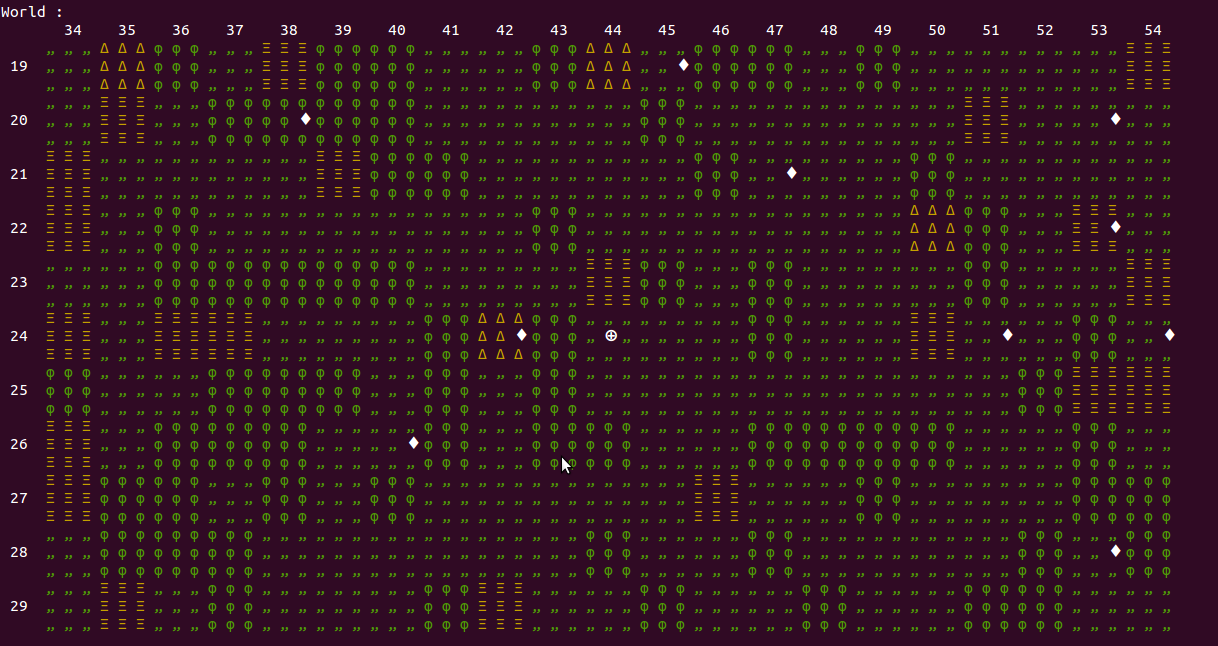
\includegraphics[width=1\textwidth]{images/screenshootCarte01.png}
    \caption{La carte du monde}	
  \end{center}
\end{figure}

Voici une explication de comment lire cette carte :
\begin{itemize}
\item chaque case du monde est représenté par un carré de 3 lignes et 3 colonnes, soit 9 symboles.
\item 4 types de terrains sont possibles : herbe, terre, forêt, et montagne. Ils sont représentés par les symboles suivants : \\
\begin{tabular}{| c c c | c c c | c c c | c c c | }
 \hline		
  \multicolumn{3}{|c|}{herbe} & \multicolumn{3}{|c|}{terre} & \multicolumn{3}{|c|}{forêt} & \multicolumn{3}{|c|}{montagne} \\	
\hline
    \verb+"+ & \verb+"+ & \verb+"+ & $\equiv$ & $\equiv$ & $\equiv$ & $\phi$ & $\phi$ & $\phi$ & $\triangle$ & $\triangle$ & $\triangle$ \\
    \verb+"+ & \verb+"+ & \verb+"+ & $\equiv$ & $\equiv$ & $\equiv$ & $\phi$ & $\phi$ & $\phi$ & $\triangle$ & $\triangle$ & $\triangle$ \\
    \verb+"+ & \verb+"+ & \verb+"+ & $\equiv$ & $\equiv$ & $\equiv$ & $\phi$ & $\phi$ & $\phi$ & $\triangle$ & $\triangle$ & $\triangle$ \\
 \hline  
 \end{tabular}
~\\
\item un objet est représenté par un $\blacklozenge$ à droite de la case.
\item un PNJ est représenté par un $\theta$ à gauche de la case.
\item le joueur est représenté par un $\bigoplus$ au centre de la case.
\end{itemize}
~\\
Vous êtes donc, dans l'exemple précédent sur la case (24, 44) et vous pouvez voir autour de vous des objets.

~\\ pour agir dans le jeu, regarder les instructions qui s'affichent en dessous de la carte.

\begin{figure}[!ht]
  \begin{center}
    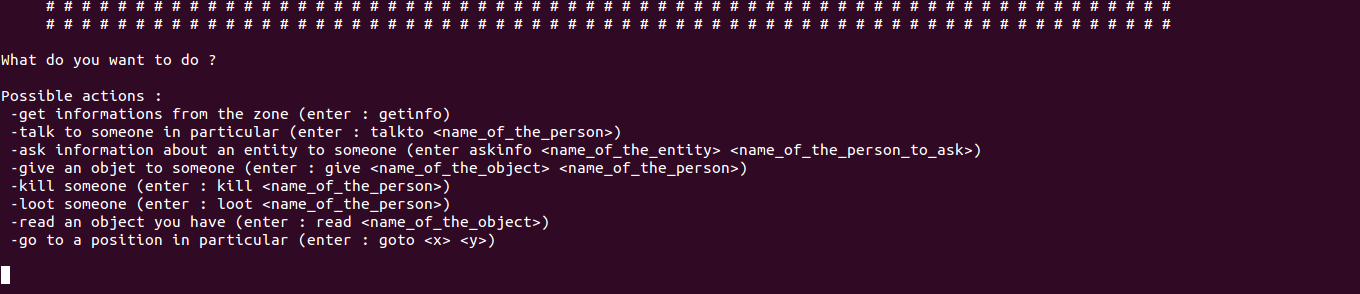
\includegraphics[width=1\textwidth]{images/screenshootUI01.png}
    \caption{Les différentes actions possibles}	
  \end{center}
\end{figure}
 vous pouvez ainsi choisir l'action que vous vouler effectuer. Par exemple pour vous déplacer, entrez : \verb+goto 24 45+. Cette action donne :
\begin{figure}[!ht]
  \begin{center}
    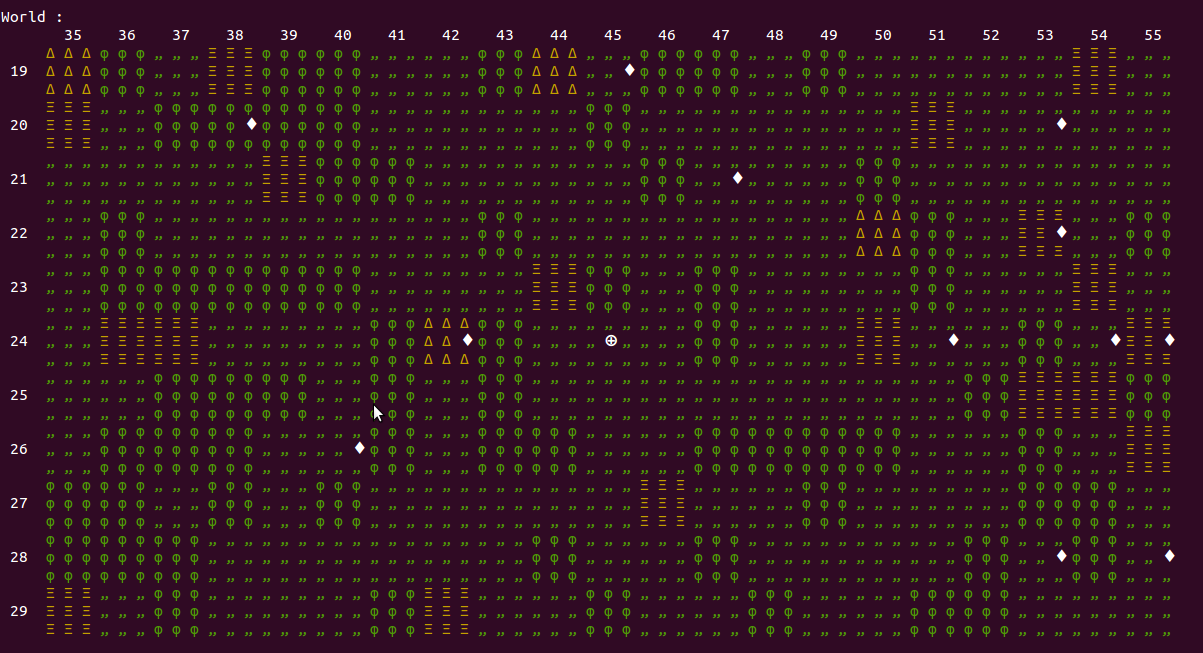
\includegraphics[width=1\textwidth]{images/screenshootCarte02.png}
    \caption{La carte du monde après avoir effectué un déplacement}	
  \end{center}
\end{figure}

Vous pouvez donc, en entrant les mots-clés correspondant effectuer les différentes actions possibles.

\end{document}
